\documentclass[11pt]{article}
\usepackage[T1]{fontenc}
\usepackage{amsmath,amssymb,amsthm}
\usepackage[margin=1in]{geometry}
\usepackage[hidelinks]{hyperref}
\usepackage{tikz}
\usepackage[ruled,vlined,linesnumbered]{algorithm2e}
\DontPrintSemicolon
\SetAlFnt{\small}
\SetAlCapFnt{\small}
\SetKw{Continue}{continue}
\SetKw{Reject}{reject}
\DeclareRobustCommand{\HullData}{\textnormal{\textsc{HullData}}}
\DeclareRobustCommand{\EndpointCode}{\textnormal{\textsc{EndpointCode}}}
\DeclareRobustCommand{\IntervalCover}{\textnormal{\textsc{IntervalCover}}}
\DeclareRobustCommand{\BatchOrders}{\textnormal{\textsc{BatchOrders}}}
\DeclareRobustCommand{\ExpectedTree}{\textnormal{\textsc{ExpectedTree}}}
\DeclareRobustCommand{\PriorityTrial}{\textnormal{\textsc{PriorityTrial}}}
\DeclareRobustCommand{\WorstTree}{\textnormal{\textsc{WorstTree}}}
\DeclareRobustCommand{\GradeDP}{\textnormal{\textsc{GradeDP}}}
\DeclareRobustCommand{\SlotDP}{\textnormal{\textsc{SlotDP}}}
\DeclareRobustCommand{\HybridTree}{\textnormal{\textsc{HybridTree}}}
\DeclareRobustCommand{\ExactTree}{\textnormal{\textsc{ExactTree}}}
\DeclareRobustCommand{\Rollout}{\textnormal{\textsc{Rollout}}}

\newtheorem{theorem}{Theorem}[section]
\newtheorem{lemma}[theorem]{Lemma}
\newtheorem{proposition}[theorem]{Proposition}
\newtheorem{claim}{Claim}[section]
\newtheorem{corollary}[theorem]{Corollary}
\theoremstyle{definition}
\newtheorem{definition}[theorem]{Definition}
\theoremstyle{remark}
\newtheorem{remark}[theorem]{Remark}
\newcommand{\HH}{\mathcal H}
\newcommand{\LL}{\mathcal L}
\newcommand{\MSSC}{\operatorname{MSSC}}
\newcommand{\OPT}{\operatorname{OPT}}
\newenvironment{symboltable}
 {\begin{center}\small
  \begin{tabular}{@{}p{0.20\linewidth}p{0.72\linewidth}@{}}
  \textbf{Symbol}&\textbf{Meaning}\\\hline}
 {\end{tabular}\end{center}}

\title{Planar Line-Query Decision Trees:\\
Approximation and Strong NP-Completeness}
\author{}
\date{October 13, 2026}

\begin{document}
\begin{figure}[htbp]
\centering
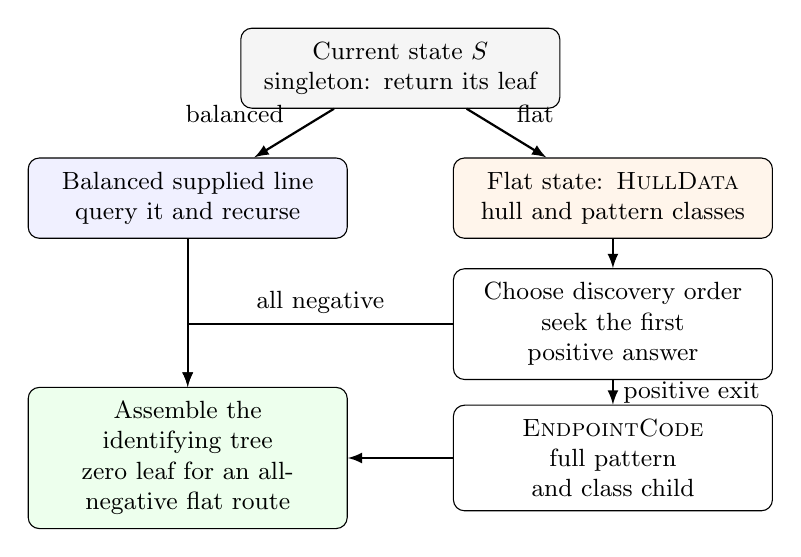
\begin{tikzpicture}[every node/.style={font=\small},
  box/.style={draw,rounded corners,align=center,inner sep=5pt,text width=3.7cm},
  arr/.style={-latex,thick}]
  \node[box,fill=gray!8] (state) at (0,0) {Current state $S$\\singleton: return its leaf};
  \node[box,fill=blue!6] (balanced) at (-2.7,-1.65)
    {Balanced supplied line\\query it and recurse};
  \node[box,fill=orange!8] (flat) at (2.7,-1.65)
    {Flat state: \HullData\\hull and pattern classes};
  \node[box] (discover) at (2.7,-3.25)
    {Choose discovery order\\seek the first positive answer};
  \node[box] (decode) at (2.7,-4.95)
    {\EndpointCode\\full pattern and class child};
  \node[box,fill=green!7] (output) at (-2.7,-4.95)
    {Assemble the identifying tree\\zero leaf for an all-negative flat route};
  \draw[arr] (state) -- node[above left]{balanced} (balanced);
  \draw[arr] (state) -- node[above right]{flat} (flat);
  \draw[arr] (flat) -- (discover);
  \draw[arr] (discover) -- node[right]{positive exit} (decode);
  \draw[arr] (discover.west) -- node[above]{all negative} (-2.7,-3.25)
    -- (output.north);
  \draw[arr] (decode) -- (output);
  \draw[arr] (balanced) -- (output);
\end{tikzpicture}
\caption{The common recursive structure. Arrows show how one stage
feeds the next. For maximum depth, the algorithm constructs class
children first and uses their heights as schedule deadlines. For
expected depth, original prior masses determine the schedule scores.
The flat stage has an all-negative leaf when the zero pattern is
present, and both scheduling and decoding use supplied hull lines.}
\label{fig:recursive-procedure-flow}
\end{figure}


\clearpage
\begin{figure}[htbp]
\centering
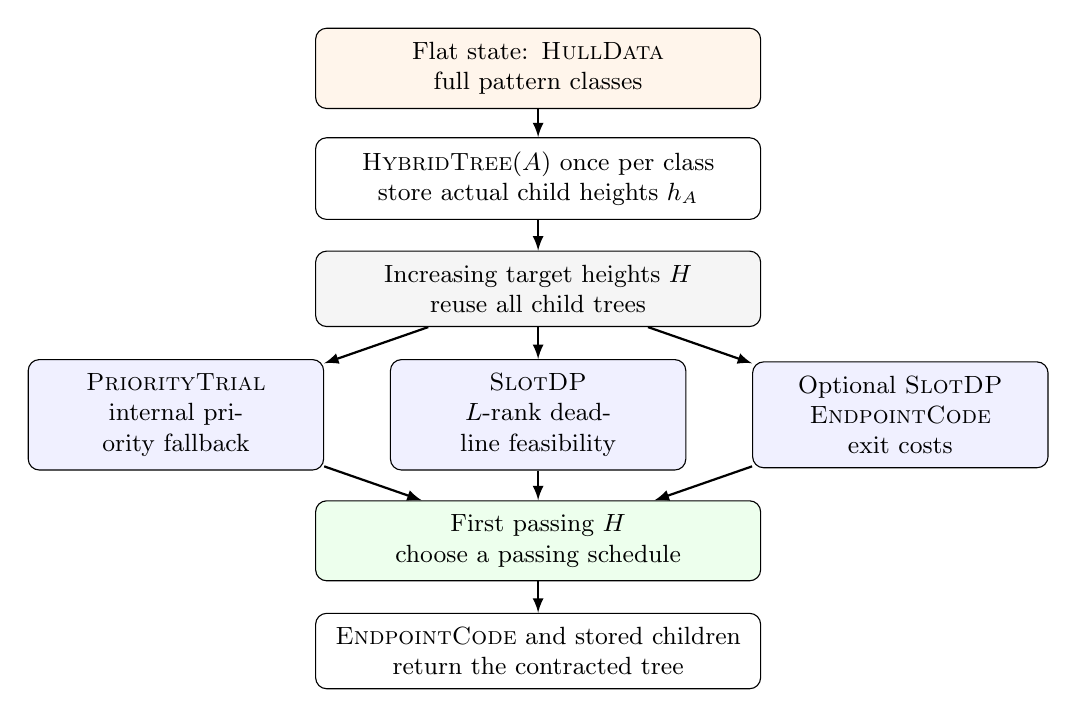
\begin{tikzpicture}[every node/.style={font=\small},
  box/.style={draw,rounded corners,align=center,inner sep=5pt,text width=3.4cm},
  wide/.style={box,text width=5.3cm},arr/.style={-latex,thick}]
  \node[wide,fill=orange!8] (hull) at (0,0)
    {Flat state: \HullData\\full pattern classes};
  \node[wide] (children) at (0,-1.4)
    {\HybridTree$(A)$ once per class\\store actual child heights $h_A$};
  \node[wide,fill=gray!8] (trial) at (0,-2.8)
    {Increasing target heights $H$\\reuse all child trees};
  \node[box,fill=blue!6] (priority) at (-4.6,-4.4)
    {\PriorityTrial\\internal priority fallback};
  \node[box,fill=blue!6] (slots) at (0,-4.4)
    {\SlotDP\\$L$-rank deadline feasibility};
  \node[box,fill=blue!6] (whole) at (4.6,-4.4)
    {Optional \SlotDP\\\EndpointCode\ exit costs};
  \node[wide,fill=green!7] (pass) at (0,-6)
    {First passing $H$\\choose a passing schedule};
  \node[wide] (attach) at (0,-7.4)
    {\EndpointCode\ and stored children\\return the contracted tree};
  \draw[arr] (hull) -- (children);
  \draw[arr] (children) -- (trial);
  \draw[arr] (trial) -- (priority);
  \draw[arr] (trial) -- (slots);
  \draw[arr] (trial) -- (whole);
  \draw[arr] (priority) -- (pass);
  \draw[arr] (slots) -- (pass);
  \draw[arr] (whole) -- (pass);
  \draw[arr] (pass) -- (attach);
\end{tikzpicture}
\caption{At a flat state, the algorithm first computes the hull and
children, then tests increasing target heights using three schedule
checks. The arrows carry the geometry, child heights, and candidate
schedules needed by those checks. The logarithmic cap $L$ is fixed at
the original root. The priority fallback guarantees a passing trial
by the stated height bound; the exact and whole-exit checks can certify
an earlier trial, and the algorithm selects the first trial accepted
by its explicit checks.}
\label{fig:hybrid-procedure-flow}
\end{figure}


\clearpage
\begin{figure}[htbp]
\centering
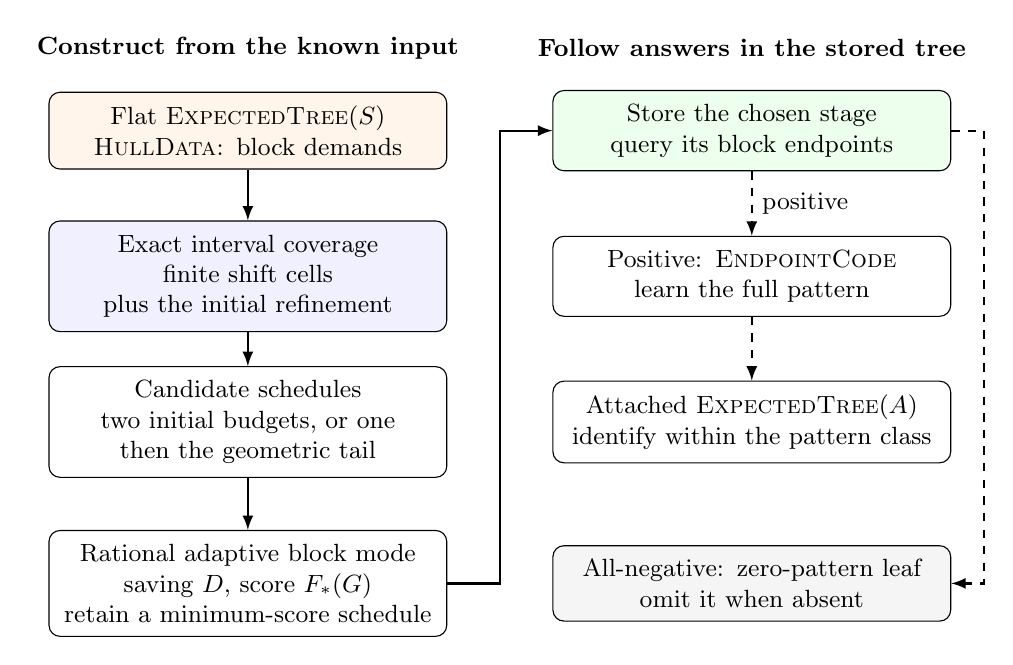
\begin{tikzpicture}[every node/.style={font=\small},
  box/.style={draw,rounded corners,align=center,inner sep=5pt,text width=4.7cm},
  arr/.style={-latex,thick},exec/.style={-latex,thick,dashed}]
  \node[font=\small\bfseries] at (-3.2,1.05) {Construct from the known input};
  \node[font=\small\bfseries] at (3.2,1.05) {Follow answers in the stored tree};
  \node[box,fill=orange!8] (hull) at (-3.2,0)
    {Flat \ExpectedTree$(S)$\\\HullData: block demands};
  \node[box,fill=blue!6] (covers) at (-3.2,-1.85)
    {Exact interval coverage\\finite shift cells\\plus the initial refinement};
  \node[box] (variants) at (-3.2,-3.7)
    {Candidate schedules\\two initial budgets, or one\\then the geometric tail};
  \node[box] (score) at (-3.2,-5.75)
    {Rational adaptive block mode\\saving $D$, score $F_*(G)$\\retain a minimum-score schedule};
  \node[box,fill=green!7] (stored) at (3.2,0)
    {Store the chosen stage\\query its block endpoints};
  \node[box] (positive) at (3.2,-1.85)
    {Positive: \EndpointCode\\learn the full pattern};
  \node[box] (child) at (3.2,-3.7)
    {Attached \ExpectedTree$(A)$\\identify within the pattern class};
  \node[box,fill=gray!8] (zero) at (3.2,-5.75)
    {All-negative: zero-pattern leaf\\omit it when absent};
  \draw[arr] (hull) -- (covers);
  \draw[arr] (covers) -- (variants);
  \draw[arr] (variants) -- (score);
  \draw[arr] (score.east) -- (0,-5.75) -- (0,0) -- (stored.west);
  \draw[exec] (stored) -- node[right]{positive} (positive);
  \draw[exec] (positive) -- (child);
  \draw[exec] (stored.east) -- (6.15,0) -- (6.15,-5.75)
    -- (zero.east);
\end{tikzpicture}
\caption{The polynomial expected-depth algorithm first computes hull
patterns and their block demands, then uses interval coverage to build
candidate schedules and selects one by its rational score. Solid arrows
show this construction-time data flow, using the supplied incidence
table and prior. The chosen stage is then stored as a query tree: dashed
arrows trace the unknown hypothesis through discovery, endpoint
decoding, and its already constructed recursive child. The adaptive
mode decides whether discovery stops at the first positive endpoint or
queries both endpoints. The algorithm makes this schedule choice
deterministically; the certificate's mixture is used to prove its cost
bound.}
\label{fig:expected-procedure-flow}
\end{figure}


\clearpage
\begin{figure}[htbp]
\centering
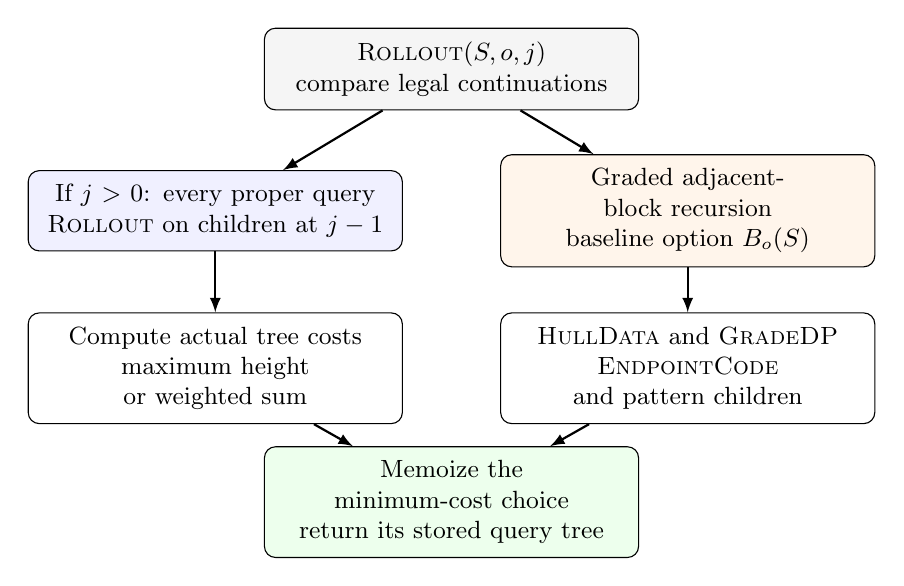
\begin{tikzpicture}[every node/.style={font=\small},
  box/.style={draw,rounded corners,align=center,inner sep=5pt,text width=4.4cm},
  arr/.style={-latex,thick}]
  \node[box,fill=gray!8] (rollout) at (0,0)
    {\Rollout$(S,o,j)$\\compare legal continuations};
  \node[box,fill=blue!6] (split) at (-3,-1.8)
    {If $j>0$: every proper query\\\Rollout\ on children at $j-1$};
  \node[box,fill=orange!8] (baseline) at (3,-1.8)
    {Graded adjacent-block recursion\\baseline option $B_o(S)$};
  \node[box] (grade) at (3,-3.8)
    {\HullData\ and \GradeDP\\\EndpointCode\ and pattern children};
  \node[box] (evaluate) at (-3,-3.8)
    {Compute actual tree costs\\maximum height or weighted sum};
  \node[box,fill=green!7] (best) at (0,-5.5)
    {Memoize the minimum-cost choice\\return its stored query tree};
  \draw[arr] (rollout) -- (split);
  \draw[arr] (rollout) -- (baseline);
  \draw[arr] (baseline) -- (grade);
  \draw[arr] (split) -- (evaluate);
  \draw[arr] (grade) -- (best);
  \draw[arr] (evaluate) -- (best);
\end{tikzpicture}
\caption{Exact lookahead wrapped around the quasipolynomial baseline.
The arrows denote calls and the returned trees or costs. The baseline
completes any branch that reaches its stopping depth. Thus the
logarithmic cap on $j$ bounds the number of search transcripts while
each returned tree still completes identification. The proof compares
this finite search with an optimal tree; the algorithm evaluates only
trees it has constructed.}
\label{fig:qp-procedure-flow}
\end{figure}

\end{document}
